\uuid{4R9m}
\chapitre{Fonction de plusieurs variables}
\niveau{L2}
\module{Analyse}
\sousChapitre{Courbes de niveaux}
\titre{Courbes de niveaux}
\theme{fonctions de plusieurs variables, courbes de niveaux}
\auteur{}
\datecreate{2023-02-23}
\organisation{AMSCC}
\difficulte{}
\contenu{

\texte{ Déterminer les courbes de niveaux des fonctions suivantes et esquisser rapidement une représentation graphique d'un ensemble de celles-ci. }
	\begin{enumerate}
		\item \question{ $f(x,y) = x+y-1$ }
		\reponse{Soit $k \in \mathbb{R}$ : $f(x,y) = k \iff y = -x+k+1$. Pour tout $k \in \R$, les lignes de niveau $k$ sont des droites de coefficient directeur $-1$. 
		
\begin{center}
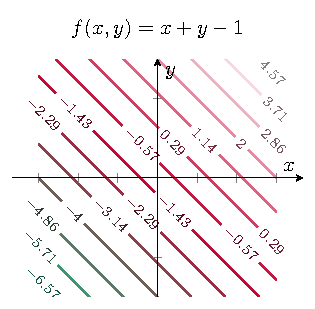
\includegraphics[]{pdf/4R9m-tikz-1}
\end{center}
}
		\item \question{ $f(x,y) = e^{y-x^2}$ }
		\reponse{Soit $k \in \mathbb{R}$ : $f(x,y) = k \Rightarrow k>0$. Pour tout $k>0$, $f(x,y) = k \iff y = x^2 + \ln(k)$. Les lignes de niveau $k>0$ sont des paraboles, vides si $k \leq 0$. 
\begin{center}
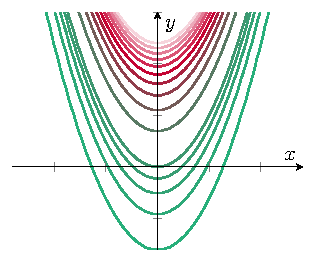
\includegraphics[]{pdf/4R9m-tikz-2}
\end{center}		
	
}
		\item \question{ $f(x,y) = \ln(x+2y)$ }
		\reponse{Soit $k \in \mathbb{R}$ : $f(x,y) = k \iff y = -\frac{x+e^{k}}{2} $. Les lignes de niveau $k$ sont des droites de coefficient directeur $-\frac{1}{2}$. 

\begin{center}
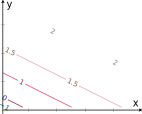
\includegraphics[]{pdf/4R9m-tikz-3}
\end{center}		
	
}
	%	\item $f(x,y,z) = \frac{\ln(x^2+1)}{yz}$
\end{enumerate}}
